%%
%% This is file `sample-sigplan.tex',
%% generated with the docstrip utility.
%%
%% The original source files were:
%%
%% samples.dtx  (with options: `sigplan')
%% 
%% IMPORTANT NOTICE:
%% 
%% For the copyright see the source file.
%% 
%% Any modified versions of this file must be renamed
%% with new filenames distinct from sample-sigplan.tex.
%% 
%% For distribution of the original source see the terms
%% for copying and modification in the file samples.dtx.
%% 
%% This generated file may be distributed as long as the
%% original source files, as listed above, are part of the
%% same distribution. (The sources need not necessarily be
%% in the same archive or directory.)
%%
%% Commands for TeXCount
%TC:macro \cite [option:text,text]
%TC:macro \citep [option:text,text]
%TC:macro \citet [option:text,text]
%TC:envir table 0 1
%TC:envir table* 0 1
%TC:envir tabular [ignore] word
%TC:envir displaymath 0 word
%TC:envir math 0 word
%TC:envir comment 0 0
%%
%%
%% The first command in your LaTeX source must be the \documentclass command.
\documentclass[sigplan,screen]{acmart}
%% NOTE that a single column version is required for 
%% submission and peer review. This can be done by changing
%% the \doucmentclass[...]{acmart} in this template to 
% \documentclass[manuscript,screen,review]{acmart}
%% 
%% To ensure 100% compatibility, please check the white list of
%% approved LaTeX packages to be used with the Master Article Template at
%% https://www.acm.org/publications/taps/whitelist-of-latex-packages 
%% before creating your document. The white list page provides 
%% information on how to submit additional LaTeX packages for 
%% review and adoption.
%% Fonts used in the template cannot be substituted; margin 
%% adjustments are not allowed.
%%
%% \BibTeX command to typeset BibTeX logo in the docs
\AtBeginDocument{%
  \providecommand\BibTeX{{%
    \normalfont B\kern-0.5em{\scshape i\kern-0.25em b}\kern-0.8em\TeX}}}

%% Rights management information.  This information is sent to you
%% when you complete the rights form.  These commands have SAMPLE
%% values in them; it is your responsibility as an author to replace
%% the commands and values with those provided to you when you
%% complete the rights form.
%\setcopyright{acmcopyright}
%\copyrightyear{2018}
%\acmYear{2018}
%\acmDOI{XXXXXXX.XXXXXXX}

%% These commands are for a PROCEEDINGS abstract or paper.
%\acmConference[Conference acronym 'XX]{Make sure to enter the correct
 % conference title from your rights confirmation emai}{June 03--05,
 % 2018}{Woodstock, NY}
%
%  Uncomment \acmBooktitle if th title of the proceedings is different
%  from ``Proceedings of ...''!
%
%\acmBooktitle{Woodstock '18: ACM Symposium on Neural Gaze Detection,
%  June 03--05, 2018, Woodstock, NY} 
%\acmPrice{15.00}
%\acmISBN{978-1-4503-XXXX-X/18/06}

%%
%% For managing citations, it is recommended to use bibliography
%% files in BibTeX format.
%%
%% You can then either use BibTeX with the ACM-Reference-Format style,
%% or BibLaTeX with the acmnumeric or acmauthoryear sytles, that include
%% support for advanced citation of software artefact from the
%% biblatex-software package, also separately available on CTAN.
%%
%% Look at the sample-*-biblatex.tex files for templates showcasing
%% the biblatex styles.
%%

%%
%% The majority of ACM publications use numbered citations and
%% references.  The command \citestyle{authoryear} switches to the
%% "author year" style.
%%
%% If you are preparing content for an event
%% sponsored by ACM SIGGRAPH, you must use the "author year" style of
%% citations and references.
%% Uncommenting
%% the next command will enable that style.
%%\citestyle{acmauthoryear}

%%
%% end of the preamble, start of the body of the document source.
\begin{document}

%%
%% The "title" command has an optional parameter,
%% allowing the author to define a "short title" to be used in page headers.
\title{A Survey of Multi-hop Reading Comprehension approaches using Graph Neural Networks}

%%
%% The "author" command and its associated commands are used to define
%% the authors and their affiliations.
%% Of note is the shared affiliation of the first two authors, and the
%% "authornote" and "authornotemark" commands
%% used to denote shared contribution to the research.
\author{Ajay Narayanan}

\author{Constantin Weberpals}

\author{Tim Bruckdorfer}


%%
%% By default, the full list of authors will be used in the page
%% headers. Often, this list is too long, and will overlap
%% other information printed in the page headers. This command allows
%% the author to define a more concise list
%% of authors' names for this purpose.
% \renewcommand{\shortauthors}{Ajay Narayanan, Constantin Weberpals, Tim Bruckdorfer}

%%
%% The abstract is a short summary of the work to be presented in the
%% article.
\begin{abstract}
  Multi-hop reading comprehension (MHRC)  has emerged as an important task in the field of Natural Language Processing. It requires the model to 
  jointly reason over multiple documents to answer a question, as well as provide supporting evidence. Although Graph Neural Networks (GNNs) 
  have been shown to be effective for this task, there have been arguments as to whether GNNs are actually necessary for MHRC.

  In this paper, we attempt to present a comprehensive survey of multi-hop reading comprehension approaches with an emphasis on 
  Graph Neural Network based approaches. We begin with a quick introduction to the MHRC task and the various approaches used to address
  the task. We then present a taxonomy of the various approaches, and discuss the core concepts of MHRC with GNNs. We then present a detailed 
  discussion on the effectiveness of graph-based approaches for MHRC and evaluate the current state of the art. Finally, we conclude with a 
  discussion of the open problems and future directions.
\end{abstract}

\maketitle

\section{Introduction}
%TODO
% Start writing your paper here and don't forget to include citations. Example: GCN \cite{RN2}
The task of Machine Reading Comprehension, or MRC is an active area of research in the field of Natural Language Processing. 
The basic goal of MRC is to develop systems that can read and comprehend unstructured passages and answer questions based on them. 

Recently, there has been a lot of interest in the task of multi-hop reading comprehension (MHRC), where the answer to a question is not 
directly stated in a single passage, but can be inferred by combining information from multiple documents. To this end, a number of datasets 
have been proposed, such as HotpotQA \cite{RN116}, QAngaroo \cite{RN115}, and MuSiQue \cite{RN167}. Some datasets also include supporting 
facts, whose extraction could be seen as providing explainability for MHRC tasks  \cite{RN116} \cite{RN106}.

To solve the task of MHRC, a number of approaches have been proposed, which can be broadly classified into two categories:
Graph-based approaches \cite{RN81} \cite{RN117} \cite{RN118} \cite{RN122} \cite{RN119} \cite{RN91} and Non-graph-based approaches. Most of 
the methods can be basically decomposed into a Retrieval phase and a Reading phase \cite{RN166}. Graph-based approaches can be effective for 
this task because they enable the modeling of complex relationships between entities \cite{RN23}, and provide the integration of global 
evidence. They can also mimic human reasoning processes \cite{RN35}.

\begin{figure}[t] % 'h' for "here", can be replaced with other placement specifiers
  \centering
  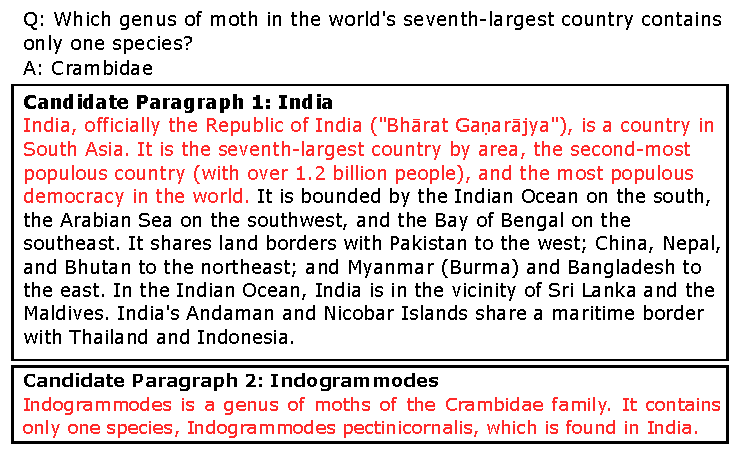
\includegraphics[width=\linewidth]{fig/fig_1_hotpot_example.pdf} % Adjust 'width' as needed
  \caption{A Sample question from the HotpotQA dataset}
  \label{fig:sample_hotpotqa} % For referencing the figure in the text
\end{figure}

%TODO: brief description of non-graph-based approaches

The first step in Graph-based approaches is to construct either an entity graph \cite{RN81} \cite{RN117} \cite{RN122} \cite{RN141} \cite{RN91}
 \cite{RN130} or a hierarchical graph \cite{RN124} \cite{RN119} \cite{RN130}, to model the relationships in the texts. Once this is done, a 
GNN-based reasoning module is used to perform multi-hop reasoning over the graph, and finally a prediction module is used to predict answers 
\cite{RN23}.
%TODO: expand this paragraph

Recently, there have been arguments as to whether GNNs are actually necessary for MHRC. Shao et al. (2020) \cite{RN127} argue that 
a graph structure may not be necessary with proper use of pre-trained models, and that the graph structure can be regarded as task-specific 
prior knowledge. Groenveld et al. (2020) \cite{RN126} showed that a simple BERT-based model can outperform a Graph-based model on the HotpotQA 
dataset, and that supporting sentence identification in HotpotQA might not be a multi-hop problem at all. Wu et al. (2021) \cite{RN106} 
suggested that the paragraph retrieval stage might be more important than the reasoning stage in MHRC, and that the reasoning stage might not 
be a multi-hop problem. Similar arguments are also made by Min et al. (2019) \cite{RN150}.
%TODO: motivation for survey - is GNN necessary for MHRC?
%TODO: mention Min et al. argument about the MHRC Dataset problem

In this paper, we present a survey of various approaches that have been proposed for MHRC, with a focus on Graph-based approaches. We also 
try to address the question of whether GNNs are actually necessary for MHRC. We first present a taxonomy of the various approaches, and then 
discuss the core concepts of MHRC. We then present a detailed discussion of the various approaches, and finally conclude with a discussion of 
the open problems and future directions.
%TODO: contributions of survey

\section{Background}
In this section we intruduce the core concepts of multi-hop reasoning and graph neural networks that prior research has established.  

%TODO
\subsection{Machine Reading Comprehension and Multi-hop QA}
The goal of MRC is to enable machines to answer questions based on a given text or set of texts, requiring a deep understanding of both the content and context of the input material, which 
requires advanced NLP techniques, such as semantic analysis, context understanding, and language modeling \cite{RN208}. MRC represents a significant challenge in AI and NLP, as it requires systems to not only process language but also to comprehend and infer meaning in a way comparable to human understanding.

Multi-hop question answering (QA) is a challanging aspect of MRC that requires multi-step reasoning over multiple passages to find the answer and supporting evidence \cite{RN165}.
It is a crucial component of natural language processing (NLP) and AI systems, with a wide range of applications, as it requires models to connect multiple pieces of 
evidence to answer complex questions. Therefore, it can be used for tasks such as document and timeline summarization \cite{RN202} \cite{RN201}.
To improve the performance of multi-hop QA models, different model architectures such as hybrid models or TransferNet, which supports both label and text relations in a unified framework \cite{RN164} \cite{RN133}. 
The development of better models was further encouraged through the availability of high quality data sets \cite{RN116} \cite{RN115}
Studies collectively highlight the importance of multi-hop QA in enhancing the reasoning and inference skills of NLP models across various domains. 
A notable development in multi-hop QA is the application of Graph Neural Networks. The multi-hop attention mechanism in GNNs, for instance, has improved information aggregation, making these 
models more effective and accurate in complex reasoning tasks \cite{RN109}. These advancements have significantly improved the performance of multi-hop QA models, making them more effective and accurate.

\subsection{Multi-hop QA Datasets}
The advancement of multi-hop QA has been greatly facilitated by the introduction of specific datasets designed to test and refine the reasoning capabilities of AI models. 
Notable among these are HotpotQA, WikiHop, and ComplexWebQuestions, each presenting unique challenges and features \cite{RN115}\cite{RN116}\cite{RN104}.
These datasets have been instrumental in benchmarking the performance and progress in the field. 



\begin{table*}[ht]
  \centering
  \begin{tabular}{|l|l|p{3cm}|p{3cm}|l|}
  \hline
  \textbf{Dataset}            & \textbf{Introduced by} & \textbf{Description} & \textbf{Key Features} & \textbf{Reasoning Types} \\ \hline
  HotpotQA           & Yang et al., 2018 & A large-scale dataset requiring understanding and synthesis of information from multiple paragraphs. & Provides questions, answers, and supporting facts for explainable QA. & Comparison, bridge, intersection \\ \hline
  WikiHop            & Welbl et al., 2018 & Constructed from Wikipedia articles, focusing on indirect inference across multiple documents. & Tests the ability to navigate and reason across linked documents. & Long-range dependencies \\ \hline
  ComplexWebQuestions & Talmor \& Berant, 2018 & Requires performing intricate queries over a large web-scale knowledge base. & Synthesizes information from various web sources. & Web-based, domain-specific knowledge \\ \hline
  \end{tabular}
  \caption{Overview of Multi-hop QA Datasets}
  \label{table:multihop_datasets}
  \end{table*}
  
  
  

\subsection{Graph Neural Networks}

A range of studies have contributed to the advancement of Graph Neural Networks (GNNs). These networks have emerged 
as a powerful tool for machine learning on graph-structured data, extending the capabilities of traditional neural networks to complex relationships and 
interdependencies encoded in graphs. The work of Gori et al. \cite{RN203} and Scarselli et al. \cite{RN204}, who proposed a framework for applying neural networks directly to graphs 
layed the foundation for further developments in that field.

GNNs are designed to capture the relational information inherent in the graphical representation of data \cite{RN205}. This makes them particularly 
well-suited for applications where data points are interrelated, such as social networks, molecular structures, and communication networks \cite{RN206}.

A core principle of GNNs lies in their ability to learn representations for nodes by incorporating neighborhood information. Through mechanisms such as neighborhood aggregation or message passing, nodes update their 
representations by adapting features from adjacent nodes \cite{RN207}. This iterative process facilitates information flow across the network, enabling the GNN to capture complex 
relational patterns \cite{RN15}. One of the most prominent variants of GNNs is the Graph Convolutional Network (GCN), introduced by Kipf and Welling (2016). 
GCNs generalize the concept of convolution from grid-like data (e.g., images) to graphs, enabling efficient feature extraction from graph data \cite{RN209}. Another notable variant is the 
Graph Attention Network (GAT), introduced by Veličković et al. (2018). GATs incorporate attention mechanisms in the aggregation process, allowing for more nuanced weighting of neighbor contributions, which 
enhances the model's ability to focus on important features in the graph \cite{RN7}.

GNNs have not only enriched the landscape of neural network architectures but have also opened new avenues in various domains that deal with complex relational data. Their continued evolution and integration with other AI fields makes them an interesting topic to investigate in the context of multi-hop reasoning.

\section{Taxonomy}
%TODO Classification theme based on different characteristics of gnns
GNNs have been effectively used for multi-hop reading comprehension, with different approaches based on certain characteristics of GNNs. In
the following, we will analyze multiple classification schemes and evaluate implemented methods building on attributes of GNNs. 

\subsection{Graph Representation}
Firstly, GNNS can be considered as representation of entities. More specifically, these entities can be associated with nodes, edges or hybrid versions. 
Li et al. (2021) \cite{RN131} introduced an Asynchronous Multi-grained Graph Network (AMGN) that represents entities and sentences as nodes, using an asynchronous 
update mechanism to mimic human multi-hop reading logic. In comparison to that, Tu et al. (2019) \cite{RN124} proposed a Heterogeneous Document-Entity (HDE) 
graph, where entities are represented as nodes and relationships as edges, and used GNNs for reasoning over this graph. Furthermore, Zhang et al. (2020) \cite{RN170} presented 
a context based Entity Graph Convolutional Network (CEG) that also represents entities as nodes, using various granularity levels of encodings and surrounding context 
to enrich entity encoding. Gao et al. (2023) \cite{RN136} introduced ClueReader, a heterogeneous graph attention network that represents entities as nodes and
relationships as edges, and uses an attention mechanism to assemble semantic features in multi-angle representations. Gao also mentions Entity-Graph 
Convolutional Network (GCN) and BAG models that focus on extracting text spans matching candidates as nodes and use contextualized word embeddings
for node representations \cite{RN136}. These studies collectively demonstrate the potential versatility of GNNs for multi-hop reading comprehension, with the
choice of entity representation as nodes or edges depending on the specific model architecture and task requirements. We find that GNNs can be adapted
to represent complex relationships between entities, documents and answer candidates in multi-hop reasoning tasks. Challenges remain in the 
interpretability and flexibility of the suggested models.

\subsection{Graph Construction}
Graph neural networks can be considered either static or dynamic, meaning that they can be constructed in a predetermined and unchangeable or flexible 
and adaptable way. In literature, the discussion primarily involves dynamic GNNs. One approach called Keywords-aware Dynamic Graph Neural Network (KA-DGN)
suggested by Jia et al. (2022) \cite{RN171b} emphasizes salient information in the text, extracting keywords from the question and context to improve MHRC performance.
The dynamic structure, in this case, allows for more adapative and responsive handling of complex questions and multiple paragraphs \cite{RN171b}. In 2022, 
Tang et al. \cite{RN172} introduced Dynamically Enhanced MHRC (DeMRC) as a method aimed at low-dataset cases. DeMRC dynamically enhances the reading comprehension process,
adapting to different datasets like the Chinese CAIL 2020 and HotpotQA. Xu et al. (2020) generally highlighting the importance of continuously inferring
clue entities and candidate answers based on the question and clue paragraphs when using dynamic GNNs for MHRC \cite{RN173}. 
As opposed to dynamic graphs, a static construction of graphs cannot deal with new or unexpected relationships in the data and hence hardly
provides an alternative. Consequently, static graph approaches are hardly of relevance in existing literature. 

% 3. Message passing
% 3.1 Aggregation techniques
% 3.2 Number of hops
\subsection{Message Passing}


% 4. Question-graph interaction
% 4.1 Query integration
% 4.2 Dynamic query graphs
\subsection{Question-Graph Interaction}

% 5. Memory augmented models
% 5.1 Graph memory networks
\subsection{Memory Augmented Models}

% 6. Datasets and Evaluation metrics
% 6.1 Benchmark datasets
% 6.2 Evaluation metrics
\subsection{Datasets and Evaluation Metrics}

% 7. Comparative Analysis
% 7.1 Comparison with Non-GNN approaches
\subsection{Comparative Analysis}
The study by Wu et al. (2021) \cite{RN106} proposes a graph-free model using a select-to-guide strategy, which outperforms all graph models on MHRC.

\section{Core Concepts}
%TODO
\subsection{An Overview of Current approaches}
For the purposes of understanding Graph based approaches, we will consider the following models:
DFGN \cite{RN122}, HGN \cite{RN119}, CogQA \cite{RN118}, Gated-RGCN \cite{RN91}, AMGN \cite{RN131} and DRN \cite{RN142}. We will also compare 
them with a couple of leading non-graph-based approaches: Beam Retriever \cite{RN105} (Current SOTA for HotpotQA Distractor Setting) and
HopRetriever \cite{RN149}.

\begin{figure*}[ht]
  \centering

 \begin{tabular} { | l | l | c | c | c | c | c | c | }
  \hline
  \multicolumn{8} { | c | }{HotpotQA Distractor Leaderboard}\\
  \hline
  \multicolumn{2} { | c | }{Model} & \multicolumn{2} { | c | }{Ans} & \multicolumn{2} { | c | }{Sup} & \multicolumn{2} { | c | }{Joint} \\
  \multicolumn{2} { | c | }{} & EM & F1 & EM & F1 & EM & F1 \\
  \hline
  1 & \textbf{Beam Retriever} \cite{RN105} & 72.69 & 85.04 & 66.25 & 90.09 & 50.53 & 77.54 \\
  3 & Smoothing R3 (single model) \cite{RN108} & 72.07 &	84.34 &	65.44 &	89.55 &	49.73 &	76.69 \\
  5 & R3 (single model) \cite{RN108} & 71.27	& 83.57	& 65.25	& 88.98	& 49.81	& 76.02 \\
  6 & SAE+ (single model) \cite{RN114} & 70.74 & 83.61	& 63.70	& 88.95	& 48.15	& 75.72 \\
  7 & S2G+EGA (single model) \cite{RN106} & 70.92	& 83.44	& 63.86	& 88.68	& 48.76	& 75.47 \\
  8 & S2G+ (single model) \cite{RN106} & 70.72	& 83.53	& 64.30	& 88.72	& 48.60	& 75.45 \\
  9 & \textbf{AMGN+} (single model) \cite{RN131} & 70.53	& 83.37	& 63.57	& 88.83	& 47.77	& 75.24 \\
 17 & HGN-large (single model) \cite{RN119} & 69.22	& 82.19	& 62.76	& 88.47	& 47.11	& 74.21 \\
 30 & C2F Reader (single model) \cite{RN127} & 67.98	& 81.24	& 60.81	& 87.63	& 44.67	& 72.73 \\
 63 & DFGN (single model) \cite{RN122} & 56.31	& 69.69	& 51.50	& 81.62	& 33.62	& 59.82 \\
 75 & \textbf{Baseline Model} (single model) \cite{RN116} & 45.60	& 59.02	& 20.32	& 64.49	& 10.83	& 40.16 \\
 
  \hline
\end{tabular}
\caption{The current leaderboard for the HotpotQA Distractor setting (\href{https://hotpotqa.github.io/}{link}). Certain models have been omitted for brevity.}
\label{fig:leaderboard_hotpotqa} % For referencing the figure in the text
\end{figure*}

\subsubsection{CogQA}
The CogQA framework \cite{RN118} is a two-stage framework, based on the \emph{Dual Process Theory} of human cognition \cite{RN137}.
The first stage is analogous to "System 1" or "Intuition", and is used to retrieve relevant information. The second stage is analogous to
"System 2" or "Reasoning", and is used to perform multi-hop reasoning over the retrieved information. A \emph{Cognitive graph} is constructed
using the extracted entities. System 2 then collects \emph{clues} which are used by System 1 to extract next-hop entities.
The Cognitive graph is initialized with the entities mention in the question $\mathcal{Q}$ and they are marked as \emph{frontier nodes}.

CogQA uses BERT \cite{RN153} for System 1. Input sentences to BERT are constructed by concatenating two functional parts 
$\text{Sentence A}$ and $\text{Sentence B}$.

$$
\underbrace{{[CLS]\: Question \: [SEP]\: clues[x; \mathcal{G}]\: [SEP]}}_{\text{Sentence A}} \underbrace{{Para[x]}}_{\text{Sentence B}}
$$

System 1 generates the semantic vector $sem[x; Q; clues]$, and pointer vectors 
$\boldsymbol{S}_{ans} , \boldsymbol{E}_{ans} $ and $\boldsymbol{S}_{hop} , \boldsymbol{E}_{hop} $ for answer and next hop spans respectively.

The primary function of System 2 is to update the hidden representations $\boldsymbol{X} \in \mathbb{R}^{n \times H}$ for all $n$ entities 
in $\mathcal{G}$. System 2 uses a variant of GNNs \cite{RN2} to perform this task. The new hidden representations $\boldsymbol{X'}$ are updated 
as follows:

$$
\Delta = \sigma((AD^{-1})^T \sigma (\boldsymbol{X}W_1))
$$
$$
\boldsymbol{X'} = \sigma(\boldsymbol{X}W_2 + \Delta)
$$

System 2 also prepares $clues[x; \mathcal{G}]$ for System 1. Finally, a two layer fully connected network is used to predict the answer.
$$
answer = \underset{\text{answer node }x}{\mathrm{argmax}}  \mathcal{F}(\boldsymbol{X}[x])
$$

\subsubsection{DFGN}
Dynamically Fused Graph Network (DFGN) \cite{RN122} constructs a \emph{dynamic entity graph}, where a dynamic local entity graph is 
constructed for each question. It is comprised of 5 modules for paragraph selection, entity graph construction, encoding, fusion 
(for multi-hop reasoning), and a final prediction layer.

The paragraph selection module for DFGN also uses a pretrained BERT-based model \cite{RN153} to select the most relevant paragraphs to the 
query $Q$ which are then concatenated to form the context $C$. Next, the entity graph is constructed with entities as nodes. The Stanford 
corenlp toolkit \cite{RN170} is used to extract entities from the context. Edges are added for sentence-level links, context-level links, 
and paragraph-level links. The query and context are concatenated and passed through a BERT-based model, and further through a bi-attention 
layer to obtain the contextualized representations.

The fusion block has 3 major steps: 1. Doc2Graph, where the text spans are converted into entity embeddings, 2. Information propagation on 
the entity graph and 3. Graph2Doc, where information passes from the entity back to the tokens. In the 2nd step, we utilize a GNN based on 
Graph Attention Networks \cite{RN7} to propagate node information. The prediction layer is similar to \cite{RN116}

\subsubsection{HGN}
Hierarchical Graph Network (HGN) \cite{RN119} proposes a hierarchical graph network with nodes for different granularity levels, like questions, 
paragraphs, sentences, and entities. Large-scale pre-trained language models like BERT \cite{RN153} or RoBERTa \cite{RN171} are used to encode 
the input text. The encoded representations are then used to construct the hierarchical graph. It uses a multi-task prediction module which 
performs multiple roles like paragraph selection, supporting fact selection, entity prediction and answer span extraction. HGN uses an 
implementation of the GAT \cite{RN7} as the GNN.

However, the model uses hyperlinks provided in the Wiki-pedia articles rather than entity linking, so it is not entirely comparable to other 
models.

\subsubsection{AMGN}
Asynchronous Multi-grained Graph Network \cite{RN131} or AMGN and it's variant AMGN+ is currently the best performing graph-based approach on the HotpotQA dataset.
The authors point out several limitations of existing GNN based approaches. Previous methods perform message-passing synchronously,
which prevents reasoning in a fine-grained logical order. Secondly, previous methods only consider the  updated entity nodes
%TODO describe previous limitations
They propose AMGN which uses an asynchronous message-passing mechanism on multi-grained nodes, which mimics the the logical order of multi-hop 
reasoning. RoBERTa \cite{RN171} is used to encode the question and the context. A heterogeneous graph is constructed with nodes for sentences 
and entities. The algorithm then performs asynchronous message-passing on the graph, dependent on the relationship level between the nodes 
(entity-entity $\to$ entity-sentence $\to$ sentence-sentence).

\subsubsection{HopRetriever}
HopRetriever \cite{RN149} is a non-graph-based approach that focuses on open-domain QA, and thus is evaluated on HotpotQA's \emph{fullwiki} 
setting. Firstly, the top 500 documents are retrieved based on their TF-IDF scores with respect to the query. The supporting documents
are then iteratively retrieved and supporting sentences are predicted from the retrieved documents. Finally, the answer is extracted 
from the supporting documents using BERT.

\subsubsection{Beam Retrieval}
 Zhang et al. (2023)\cite{RN105} introduce Beam Retrieval, which is a retrieval approach that uses a beam search to retrieve the relevant 
 paragraphs. It keeps multiple hypotheses in consideration at each step, and is thus suited for questions requiring variable hop reasoning. 
 A Supervised Reader or a zero-shot LLM is used for the reading module. It achieves strong performance and has achieved SOTA on the 
 HotpotQA dataset \cite{RN116}.


\subsection{Evaluating the effectiveness of Graph-based approaches}

For a long while, Graph based approaches were seen as the SOTA for MHRC. However, recently, there have been arguments as to whether GNNs 
are actually necessary for MHRC. The best performing models on the HotpotQA dataset \cite{RN116} are non-graph-based approaches \cite{RN105} 
\cite{RN149}.

Min et al. (2019) \cite{RN150} argue that constructing large multi-hop datasets is difficult, and that the current datasets like HotpotQA can 
be solved with single-hop approaches. They also suggest that more focus should be given to the retrieval stage, and that the reasoning stage, 
atleast for current datasets might not be a multi-hop problem. They noted that humans could solve over 80\% of HotpotQA questions with one 
gold paragraph withheld. This indicates that current datasets may not be suitable for evaluating the effectiveness of graph-based approaches.

Shao et al. (2020) \cite{RN127} argue that a graph structure may not be necessary with proper use of pre-trained models, and that the graph 
structure can be regarded as task-specific prior knowledge. For their approach, they reimplement DFGN \cite{RN122} as their baseline to perform 
their evaluations. They use RoBERTa \cite{RN171} to retrieve paragraphs, and to encode query and context A fine-tuned pre-trained BERT Model 
is used to extract entities from candidate paragraphs. They compare the results with the fusion block, and also by removing the fusion block 
and directly feeding the outputs of the pre-trained layer directly to the prediction layer. They find that by using a fine-tuning approach, 
models with and without graph fusion block can reach almost equal results. They also point out that Graph 
attention is a special case of self-attention, which is to be noted as in the leaderboard, the best performing graph-based approaches tend 
to use GATs.

Groenveld et al. (2020) \cite{RN126} showed that a simple BERT-based model can outperform a Graph-based model on the HotpotQA dataset.
Their results show that a simple model that identifies relevant paragraphs independent of each other performs unexpectedly well, as compared to 
jointly identifying the paragraphs through methods like graph networks. Their results indicate that HotpotQA might not be suitable to 
demonstrate the value of more complex retrieval techniques, and that supporting sentence identification in HotpotQA might not be a multi-hop 
problem at all.

Wu et al. (2021) \cite{RN106} models the multi-hop reasoning nature in the retrieval module rather than the reader module, avoiding the need 
for a graph-based reasoning module. It highlights the limitations of graph modeling for MHRC, which requires Named Entity Recognition and 
also requires rigid rule-based graph construction. They also point out that retrieval of evidence paragraphs is essentially a ranking problem 
rather than individual sequence classification. They also consider the multi-hop nature of paragraph retrieval and that secondary evidence 
extraction is usually dependent on the previous evidence. The Select-to-Guide (S2G) model outperformed all graph-based models reaching new 
SOTA on HotpotQA.


%TODO: add a table summarizing the results of the various approaches if applicable on same dataset

\subsection{Analysis of Multi-hop Datasets}
%TODO graph based models are still pretty good in the fullwiki setting - maybe that is a potential future direction?

HotpotQA seems to be the de-facto dataset for evaluating MHRC models. However, there have been arguments that the dataset itself is flawed. 
Several studies \cite{RN176} \cite{RN175} \cite{RN154} \cite{RN150} indicate that many questions in HotpotQA can be answered using heuristics, 
as they have biases and reasoning shortcuts \cite{RN177}.



\section{Related Work}
%TODO

\section{Conclusion}
%TODO Dive into current challenges and give a brief outlook on future work and research gaps that need to be addressed 

% add bibliography
\bibliographystyle{ACM-Reference-Format}
\bibliography{bib.bib}

\end{document}
\endinput
%%
%% End of file
